%!TEX root = mb.tex

\section{System implementation} \label{sec:impl}
\eat{
\todo{this is important to write properly because it is a systems paper and there were some nontrivial decisions}.

Things to cover:

- gateway and middlebox implementation

- explain why the firewall hardware does not change (or was that above?)

- second flow udp/tcp

- might want to explain these points made in intro: "
Sylvia, it would be great if you could read and revise the paper. Feel free to edit directly in tex!
We really need your feedback at this stage."

- new packet structure and headers -- multiple layers of headers? graph? (there is some text and a figure in a google doc about this)

- some things are specific to web proxy from what I remember
}

We now describe the \sys architecture and implementation. 
As discussed in \S\ref{sec:overview}, \sys redirects traffic to the cloud and back for {\it middlebox processing} using a {\it redirection gateway}.
We now present the implementation and architecture of the redirection gateway (\S\ref{sec:gateway}), followed by the modifications we made to middleboxes to support \sys (\S\ref{sec:middleboxes}).
Finally, we discuss our EC2 deployment of these components (\S\ref{sec:deployment}).


\subsection{Redirection \& gateway implementation}
\label{sec:gateway}

\begin{figure}[t]
  \centering
  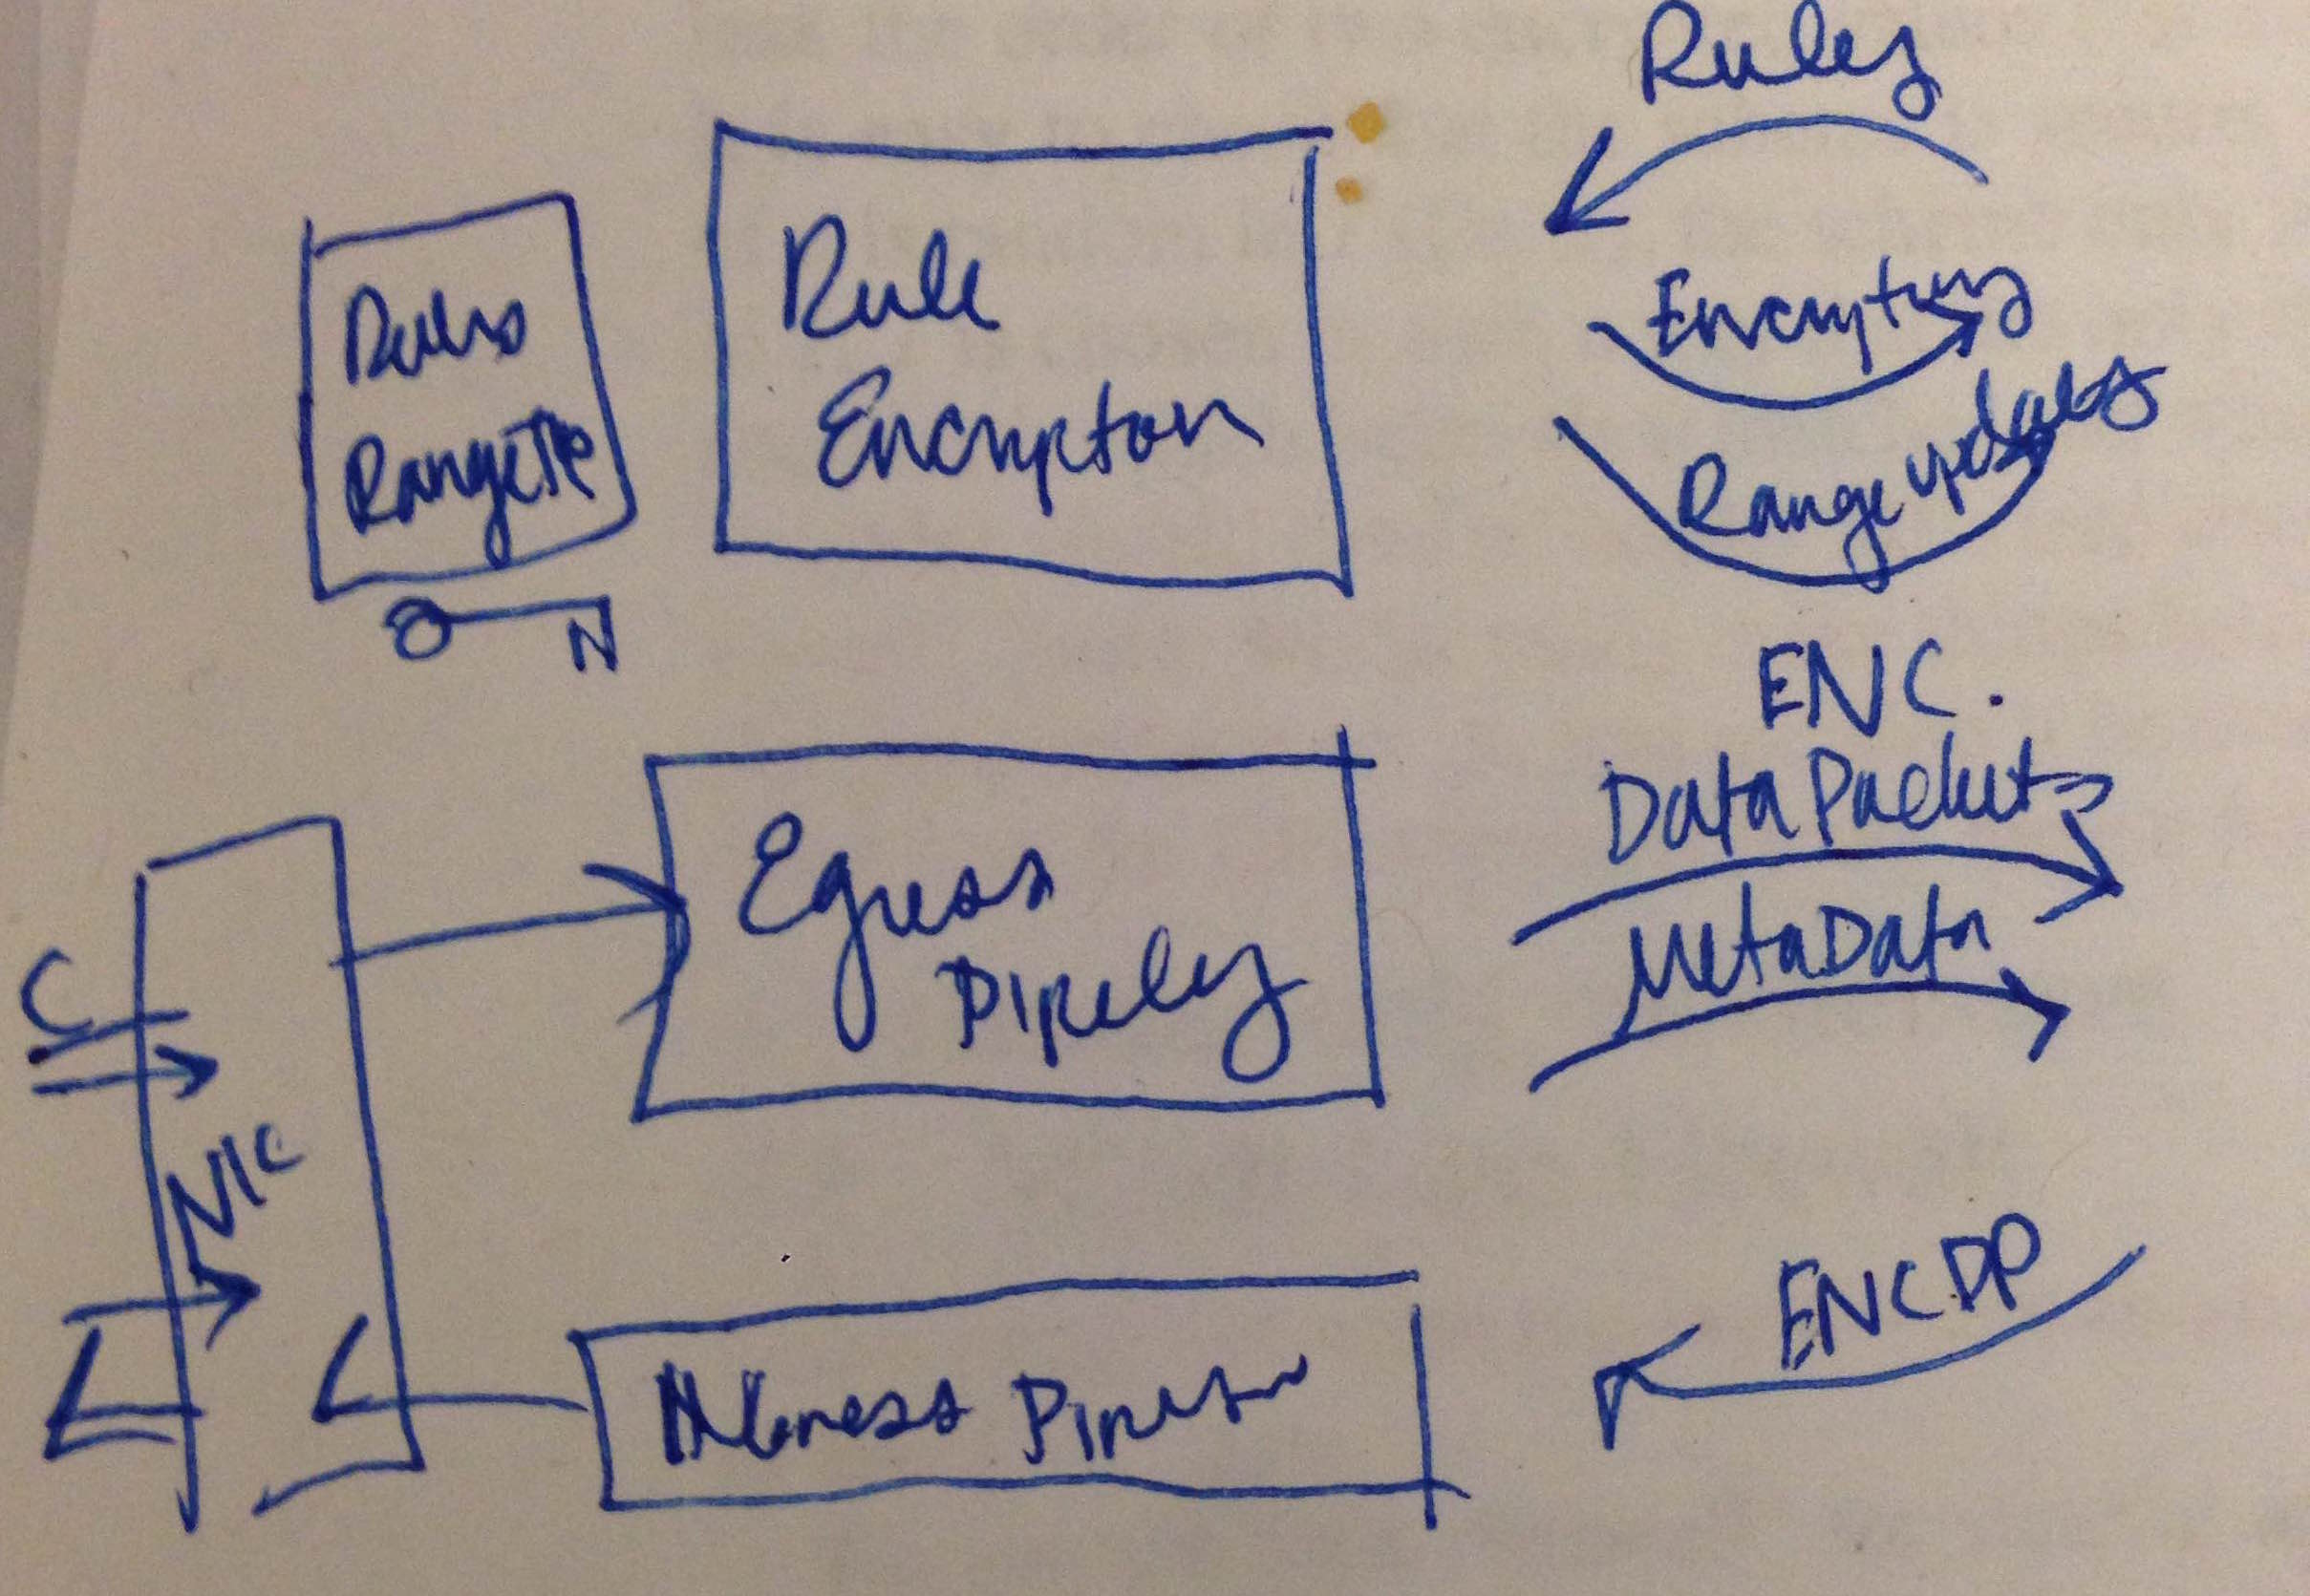
\includegraphics[width=3.25in]{fig/gatway_metaarch.JPG}
  \caption[]{\label{fig:gatewaymeta} Communication between the cloud and three gateway services: rule encryption, data encryption, and data decryption}
\end{figure}



\begin{figure}[t]
  \centering
  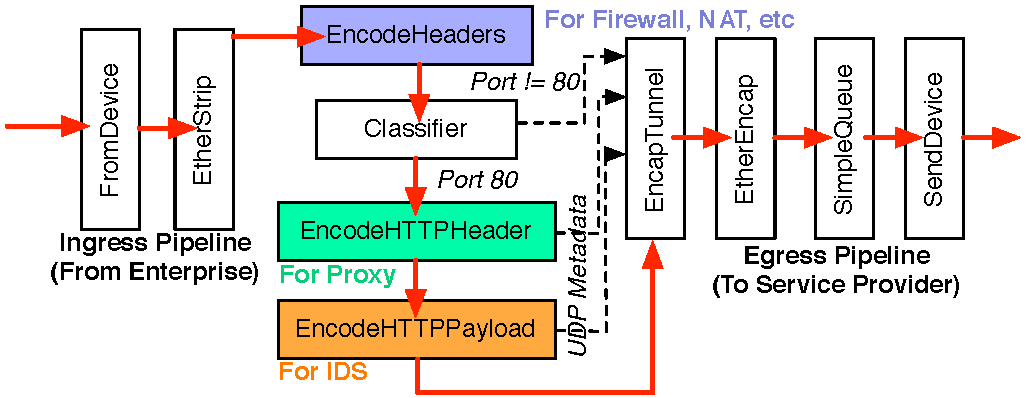
\includegraphics[width=3.25in]{fig/gatewaydiag}
  \caption[]{\label{fig:gateway} Enterprise to service provider packet processing pipeline.}
\end{figure}

The gateway serves two purposes. First, it redirects traffic to/from the cloud for middlebox processing. Second, it provides the cloud with encryptions of IDS/FW rulesets and updates to the RangeMatch tree.
Every gateway is configured statically to tunnel traffic to a fixed IP address at a single service provider point of presence.
A gateway can be logically thought of as three services: the rule encryption service, the pipeline from the enterprise to the cloud (Data encryption), and the pipeline from the cloud to the enterprise (Data decryption). 
All three services share access to the RangeMatch tree and the private key $k$.
Figure~\ref{fig:gatewaymeta} illustratres  these three services and the data they send to and from the cloud provider.

\noindent{\bf Rule Encryption.} The rule encryption component provides the cloud provider with encrypted rules/policies to use at the middlebox. 
There are two possible ways rules can be generated. First, an enterprise may choose to generate their own rules, in which case, they send encrypted versions of the rules directly to the cloud.
Rules can contain IP addresses, port numbers, and substrings of attack signatures; the first two must be encrypted with both keyword match and range match, the last needs only to be encrypted with keyword match.
Alternately, the enterprise may opt in to a `default' set of rules from the cloud provider, in which case the cloud provider sends the rules to the gateway which encrypts them and sends them back.
The rule encryption component also sends update. Whenever an adjustment is made to the RangeMatch table, it sends an update to the cloud provider with the adjusted mappings/rules.
If the gateway ever changes its key, the encryption component must also signal to the cloud provider and re-encrypt all rules.
\todo{too high level? Details about how updates work?}

\noindent{\bf Data Encryption.} In Figure~\ref{fig:gateway}, we show the DPDK-Click~\cite{click} packet processing pipeline that implements data encryption and transmits packets from the enterprise to the cloud.
This figure assumes the enterprise is already using IPv6, if it is not, the pipeline would also include a `4to6' element.
In \S\ref{sec:overview}, we described how \sys encodes packet content using the AES, Keyword Match, and Range Match encryption algorithms. 
The encrypted values are placed either directly back in to a data packet, or transmitted over a {\it metadata channel}.

Below, we detail the three elements we implemented to encrypt the packet data:

\noindent {\it Encode Headers:} Encrypts the IP, TCP, and UDP headers, replacing all IP and Port numbers in the packet with values calculated using the {\it RangeMatch} encryption algorithm. Appends the AES-encrypted values to the IP options field of the data packet.
Required to support all middleboxes. 

\noindent {\it Encode HTTP Header.} Encrypts the HTTP header for {\it the first GET request only.} Does not modify the data packet itself, but instead places the keyword match encryptions of the values in a new packet sent over the metadata channel. 
The new packet marks (a) the encrypted 5-tuple flow ID for the packet, (b) that this is HTTP GET data for the proxy, and (c) the encrypted values. At the cloud, the proxy can read this metadata channel to obtain the encrypted URL for the GET request and check its cache for the encrypted data. This element is only needed if there is an HTTP proxy enabled at the cloud, otherwise it can be disabled at the gateway.

\noindent {\it Encode HTTP Payload.} Encrypts the entire HTTP payload (as described in \S\ref{sec:ids}), placing the keyword match values in a new packet in the metadata channel. Unlike the other two elements, this element keeps per-flow state, reconstructing the TCP stream in order to generate keyword match tokens for keywords which are divided across two subsequent packets.  The metadata channel packets contain (a) the encrypted 5-tuple for the packet, (b) that the packet contains keyword match data for the IDS, and (c) the encrypted values. At the cloud, the IDS can read this metadata channel to detect attacks; if there is a match it instructs the firewall to block the 5-tuple for the flow. This element is only needed if there is an IDS enabled at the cloud, otherwise it can be disabled at the gateway.


\noindent{\bf Data Decyption.} Packets returning from the cloud follow a much simpler packet processing pipeline than those being encrypted.



\subsection{Middlebox Implementations}
\label{sec:middleboxes}

\begin{figure}[t]
  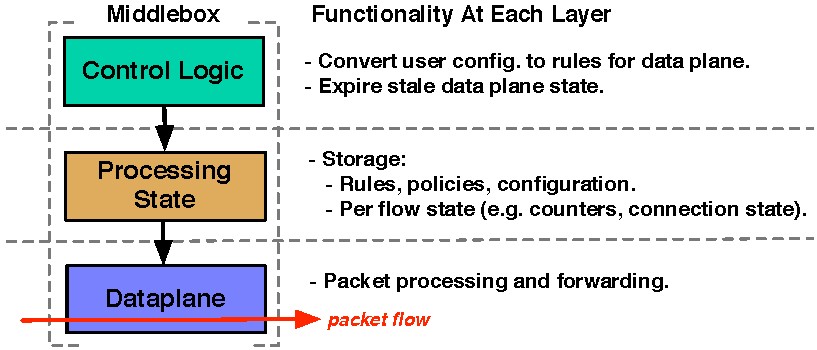
\includegraphics[width=3.25in]{fig/mbarch}
  \caption[]{Typical middlebox software architecture. To be compatible with \sys, most middleboxes only require changes in the control logic. For these devices, packet processing operations in the dataplane remain unmodified and performance-competitive.}
\end{figure}

\subsection{Unmodified Middleboxes}
\begin{itemize}
  \item IP Firewall, NAT, IP Forwarding, LB L4
  \item Operations: Match, Match/Replace, Range -- on specific fields
  \item Why no change? Packets are valid IPv6 packets, and all we need to do is have encrypted rules as well.
  \item How rules are encrypted, how often rules must be updated for Range (basically never) which we show in eval.
\end{itemize}

\subsubsection{Modified Middleboxes}
\begin{itemize}
  \item Exfiltration, IDS, Proxy, App Firewall, L7 Load Balancer
  \item Why change? All perform some kind of DPI -- variable offset, and variable operation. Key thing we need is the match, but the encoding that comes out looks very different than the normal packet.
  \item Required modifications:
    \begin{itemize}
      \item Exfiltration, IDS, App Firewall -- same as BB
      \item Proxy -- mapping from crypto to table. Note that the session termination code -- which is complicated! -- does not change at all because these are all header operations on what looks liek a valid IPv6 packet.
      \item L7 Load Balancer -- I actually don't know how this one works?
    \end{itemize}
\end{itemize}

\subsection{Deployment}
\label{sec:deployment}
